%!TEX root = ../../thesis.tex
\chapter{基盤モデルを用いたシナリオ駆動型ナビゲーションシステム}
\label{chap:method}

本章では，基盤モデルを用いたシナリオ駆動型ナビゲーションのシステムについて述べる．
まずシステムの全体像とナビゲーションの流れを示し，次に設計方針と各モジュールの詳細を述べる．

\section{システムの概要}
\label{sec:system}

システムの構成を\figref{fig:system}に示す．
システムは，次の3つのモジュールから構成される．
\begin{itemize}
  \item シナリオモジュール：人間が「次の角まで直進．左折．」のような自然言語に近い定型表現で記述した道順を，条件と行動の組に分解する．現在の行動を目標方向として経路追従モジュールへ与え，通路分類の結果から条件の成立を判定する．
  \item 通路分類モジュール：観測画像から角や交差点などの通路形状を推定する．
  \item 経路追従モジュール：観測画像と目標方向に基づいてwaypoint列を生成し，ロボットを通路に沿って走行させる．
\end{itemize}
いずれのモジュールも，実行時の入力は単眼RGBカメラの画像のみであり，地図や自己位置は用いない．

\begin{figure}[tb]
  \centering
  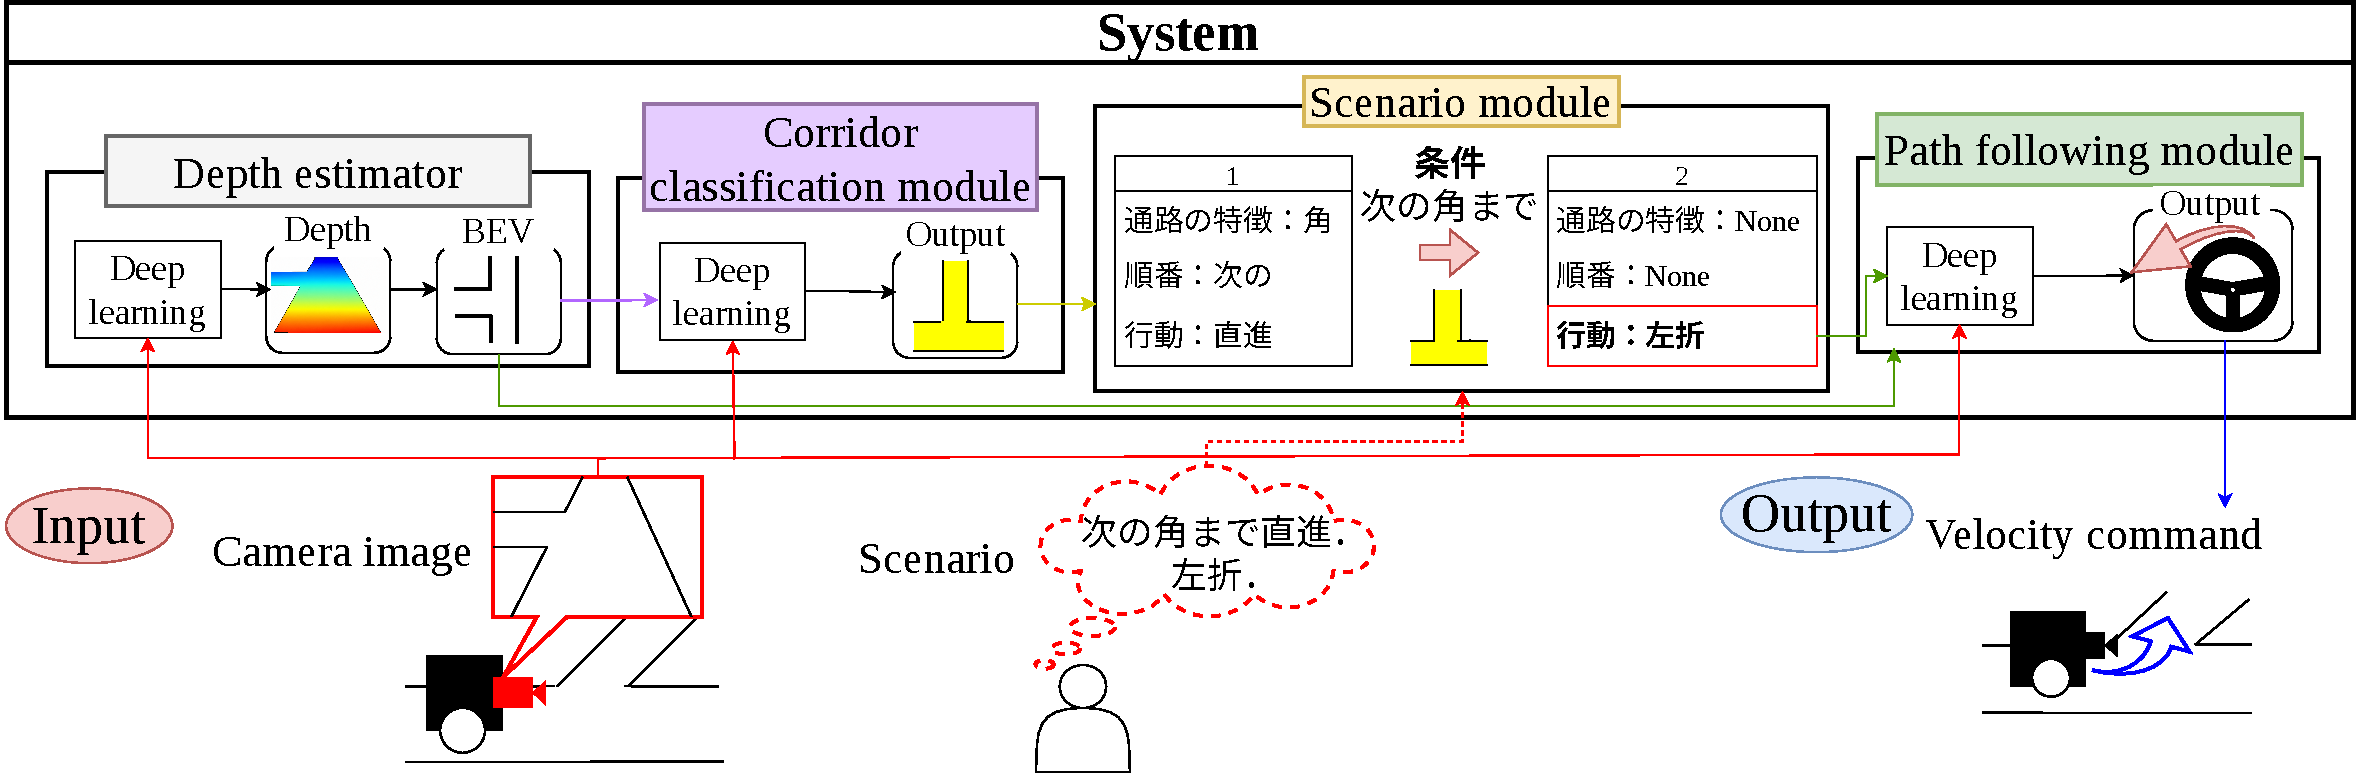
\includegraphics[width=\linewidth]{images/system.pdf}
  \caption{Scenario-driven navigation system}
  \label{fig:system}
\end{figure}

\section{ナビゲーションの流れ}
\label{sec:flow}

ナビゲーションの流れを以下に示す．
ロボットは，（a）で記述したシナリオを（b）で分解したのち，（c）から（e）を繰り返すことで，シナリオで指示された経路に沿って自律移動する．
\begin{enumerate}[label=（\alph*）,leftmargin=*,labelsep=0pt]
  \item 人間が，目的地までの道順を条件と行動の組として記述する．例えば，「次の角まで直進．左折．」というシナリオを作成する．
  \item シナリオモジュールがシナリオを分解し，条件と行動を抽出する．上記の例では，「次の角まで」を条件，「直進」を行動として取得する．
  \item シナリオモジュールが「直進」を目標方向として経路追従モジュールへ与え，経路追従モジュールはこの目標方向に沿ってロボットを走行させる．
  \item ロボットが角へ接近すると，通路分類モジュールが通路形状を「角」と分類する．シナリオモジュールは分類結果から「次の角まで」という条件が成立したと判定し，次の行動へ遷移する．
  \item シナリオモジュールが「左折」を新たな目標方向として経路追従モジュールへ与える．経路追従モジュールは新しい目標方向に従って角を左折する．
\end{enumerate}

\section{設計方針}
\label{sec:policy}

本研究では，ファインチューニングに用いていない環境においても，目的地まで移動可能かを調査する．
そのため，通路分類と経路追従には大規模データで事前学習された基盤モデルを用い，単一の環境で収集したデータによるファインチューニングで事前学習の表現が損なわれないようにする．
具体的には，基盤モデルの特徴抽出器を凍結し，主に新たに追加した部分を学習する．

単一の環境で収集したデータは，床や壁の色，照明などの外観が限られている．
このデータで特徴抽出器まで更新すると，モデルが学習環境の外観に依存した特徴を獲得し，外観の異なる環境で性能が低下するおそれがある．
特徴抽出器を凍結し，追加した小さな部分だけを学習すれば，事前学習で獲得された汎用的な表現をそのまま利用しつつ，本研究のタスクに必要な出力を得られると考える．
また，見た目に依存しにくい幾何的な情報として，単眼深度推定の結果を併用する．

\section{シナリオモジュール}
\label{sec:scenario_module}

シナリオモジュールは従来手法\cite{scenario_si2023}から変更していない．
シナリオの各文は1つの状態に対応し，各状態は「通路の特徴」「順番」「行動」の3要素で表される（\figref{fig:system}）．
例えば，「次の角まで直進．」は，通路の特徴を「角」，順番を「次の」，行動を「直進」とする状態となる．
通路の特徴と順番は状態の終了条件を表し，行動は目標方向を表す．
シナリオモジュールは，通路分類結果が終了条件を満たすと次の状態へと遷移し，新しい目標方向を経路追従モジュールへ送る．
目標方向は，直進，左折，右折の3通りである．

シナリオの文は形態素解析により単語に分割し，あらかじめ定めた語彙と照合して各要素を取り出す．
シナリオで用いる語彙を\tabref{tab:scenario_vocabulary}に示す．
通路の特徴には「左手に」「右手に」のように方向を付けることができ，「左手に通路が見えるまで直進．」は，左側に分岐が現れるまで直進することを表す．
順番は「3番目の三叉路まで」のように数で指定し，省略した場合は次に現れる通路を対象とする．

\begin{table}[tb]
  \centering
  \caption{Vocabulary of the scenario}
  \label{tab:scenario_vocabulary}
  \begin{tabular}{lp{0.7\linewidth}}
    \toprule
    要素 & 語彙 \\
    \midrule
    通路の特徴 & 一本道，三叉路，行き止まり，十字路，突き当り，曲がり角，角，通路，交差点 \\
    方向 & 前，前方，右，右手，左，左手，後ろ，後方 \\
    順番 & 〜つ目，〜番目，次 \\
    行動 & 直進，前進，右折，左折，向く，曲がる，停止 \\
    \bottomrule
  \end{tabular}
\end{table}

% TODO: 語彙は scenario_navigation/scripts/scenario_parser_jsk.py から取った．
%       「突き当り」と「行き止まり」の違いなど，条件判定の規則（cmd_dir_executor_detailed.cpp）を確認して書き足す．

\section{通路分類モジュール}
\label{sec:corridor_classifier}

\subsection{概要}

通路分類モジュールの構成を\figref{fig:corridor_classifier}に示す．
本モジュールは，直進方向，右分岐，左分岐の有無を推定し，その組合せから通路形状を出力する．
例えば，直進方向と右分岐が存在し，左分岐が存在しないと判定した場合，「三叉路右」という通路形状を出力する．
3方向の有無と通路形状の対応を\tabref{tab:passage_directions}に示す．
通路形状を直接分類するのではなく，3方向の有無を独立に推定することで，それぞれの出力が画像中の左，中央，右の領域の見え方と対応し，学習データの少ない通路形状でも各方向の判定を共有できる．

\begin{table}[tb]
  \centering
  \caption{Passage classes and the presence of each direction}
  \label{tab:passage_directions}
  \begin{tabular}{lccc}
    \toprule
    Passage class & Front & Left & Right \\
    \midrule
    straight\_road & \checkmark & & \\
    3\_way\_left   & \checkmark & \checkmark & \\
    3\_way\_right  & \checkmark & & \checkmark \\
    3\_way\_center & & \checkmark & \checkmark \\
    cross\_road    & \checkmark & \checkmark & \checkmark \\
    corner\_left   & & \checkmark & \\
    corner\_right  & & & \checkmark \\
    dead\_end      & & & \\
    \bottomrule
  \end{tabular}
\end{table}

% TODO: 表の対応はクラス名から整理したもの．corridor_classifier の実装と一致するか確認する．

\begin{figure}[tb]
  \centering
  \resizebox{\linewidth}{!}{% 通路分類モジュールの詳細図．paper.tex から \input して使う．
% 画像・BEV は未学習環境 m の実データおよび UniDepth の実出力．
% 各ブロックは隣のブロックからの間隔（\gap）で配置する．
\begin{tikzpicture}[
    font=\normalsize,
    blk/.style={draw, align=center, minimum height=8mm, minimum width=16mm,
                inner xsep=2pt},
    val/.style={draw, align=center, minimum height=6.5mm, minimum width=10mm},
    pic/.style={draw, inner sep=0pt},
    grp/.style={draw, dashed, gray},
    frz/.style={fill=cyan!12},
    lbl/.style={font=\small, inner sep=1.5pt},
    ar/.style={-{Latex[length=1.6mm]}, thin},
]
\def\gap{3mm}
% BEV 枝は UniDepth から 128-D までを等間隔にする（上段の幅から決めた値）．
\def\botgap{7.4mm}
% 各行の高さ
\coordinate (top) at (0,0);
\coordinate (mid) at (0,-1.8);
\coordinate (bot) at (0,-3.6);

% ---- 入力 ----------------------------------------------------------------
\node[pic] (rgb) at (0,-1.7) {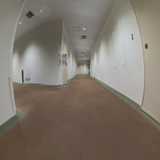
\includegraphics[width=13mm]{images/cc_rgb.png}};
\node[lbl, below=0.5mm of rgb] {RGB image};
\coordinate (rsplit) at ([xshift=2.5mm]rgb.east);

% ---- RGB 枝 --------------------------------------------------------------
\node[blk, anchor=west] (res) at ([xshift=\gap]rsplit |- top) {Resize\\$224\times224$};
\node[blk, frz, right=\gap of res] (dno) {\DINOvTwo\ ViT\text{-}S/14\\\small \frozen};
\node[blk, right=\gap of dno] (rdo) {Spatial readout\\\small CLS $+$ 3 regional means};
\node[val, right=\gap of rdo] (f15) {$1536$\text{-}D};
\node[pic] (b2) at (rdo |- 0,-1.4) {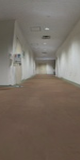
\includegraphics[width=6mm]{images/cc_band2.png}};
\node[pic] (b1) at ([xshift=-7mm]b2) {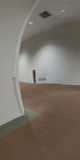
\includegraphics[width=6mm]{images/cc_band1.png}};
\node[pic] (b3) at ([xshift=7mm]b2) {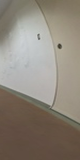
\includegraphics[width=6mm]{images/cc_band3.png}};
\node[lbl, below=0.5mm of b2] {left \,\textbar\, center \,\textbar\, right};

% ---- BEV 枝 --------------------------------------------------------------
\node[blk] (udp) at (res |- bot) {\UniDepth};
\node[pic, right=\botgap of udp] (dep) {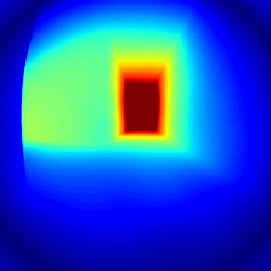
\includegraphics[width=11mm]{images/pf_depth_cmap.png}};
\node[pic, right=\botgap of dep] (bev) {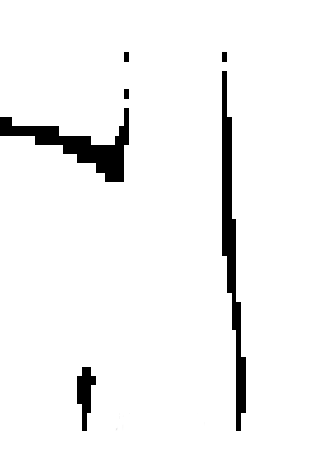
\includegraphics[height=15mm]{images/cc_bev_inner.png}};
\draw (bev.south west) rectangle (bev.north east);
\node[lbl, below=0.5mm of bev] {BEV $50\times70$};
\node[blk, right=\botgap of bev] (cnn) {BEV CNN\\\small $4\times4$ pooling};

% ---- 分類ヘッド ----------------------------------------------------------
% 1536-D と 128-D は Feature fusion の真上と真下に置き，縦の矢印で結ぶ．
\node[blk] (fus) at (f15 |- mid) {Feature fusion\\\small $256$\text{-}D};
\node[val] (f12) at (f15 |- bot) {$128$\text{-}D};
\node[blk, right=\gap of fus] (gru) {GRU\\\small 3 frames, stride 4};
\node[blk, right=\gap of gru] (lin) {Linear $+$\\sigmoid};
\node[val, minimum width=13mm, right=4mm of lin] (pr) {$p(\mathrm{right})$};
\node[val, minimum width=13mm, above=2.5mm of pr] (pf) {$p(\mathrm{front})$};
\node[val, minimum width=13mm, below=2.5mm of pr] (pl) {$p(\mathrm{left})$};

% ---- 結線 ----------------------------------------------------------------
\draw[thin] (rgb.east) -- (rsplit);
\draw[ar] (rsplit) |- (res.west);
\draw[ar] (rsplit) |- (udp.west);
\draw[ar] (res) -- (dno);
\draw[ar] (dno) -- (rdo);
\draw[ar] (rdo) -- (f15);
\draw[ar] (udp) -- (dep);
\draw[ar] (dep) -- (bev);
\draw[ar] (bev) -- (cnn);
\draw[ar] (cnn) -- (f12);
\draw[ar] (f15) -- (fus);
\draw[ar] (f12) -- (fus);
\draw[ar] (fus) -- (gru);
\draw[ar] (gru) -- (lin);
\draw[ar] (lin.east) -- (pf.west);
\draw[ar] (lin.east) -- (pl.west);
\draw[ar] (lin.east) -- (pr.west);

\end{tikzpicture}
}
  \caption{Corridor-classification module}
  \label{fig:corridor_classifier}
\end{figure}

\subsection{RGB画像の特徴}

視覚特徴の抽出には\DINOvTwo を用いる．\DINOvTwo のパラメータは学習時にすべて凍結し，大規模データによる事前学習で獲得された視覚表現を保持する．
単一の棟で収集したデータに対して特徴抽出器まで更新すると，学習環境の外観に過度に適合するおそれがあるためである．

モデルにはViT-S/14を用い，入力画像は$224\times224$にリサイズする．
最終層のCLSトークンに加え，パッチトークンを画像の左，中央，右の3つの縦長の領域に分けて領域ごとに平均する．
CLSトークンは画像全体の特徴を表すが，分岐がどちら側にあるかという位置の情報は失われやすい．
領域ごとの平均を併用することで，左右の分岐の有無を判定するための位置の情報を保持する．
CLSトークンと3つの領域の平均はそれぞれ384次元であり，これらを結合した1536次元のベクトルをRGB画像の特徴とする．

\subsection{鳥瞰の占有格子}

また，見た目に依存しにくい情報として，\UniDepth により推定した深度から床面と天井を除いた壁面および障害物の点群を求め，水平面へ投影した鳥瞰（BEV: Bird's-Eye View）の占有格子を併用する．
具体的には，推定深度から求めた点群のうち，高さ$\SI{0.05}{m}$から$\SI{1.6}{m}$の点を壁面および障害物とする．
これらの点を，前方$\SI{0.1}{m}$から$\SI{5.1}{m}$，左右$\pm\SI{3.5}{m}$の範囲で，一辺$\SI{0.1}{m}$の格子に投影し，$50\times70$の占有格子を作成する．
各格子には，点が存在するかどうかを2値で与える．
点の数をそのまま用いると，カメラからの距離や壁面の材質によって値が変わるためである．

占有格子は小さなCNNで処理し，出力を$4\times4$の領域ごとに平均して128次元の特徴とする．
格子全体を1つの値に平均すると，通路の開口部がどこにあるかという情報が失われるため，領域ごとに平均して位置の情報を残す．

\subsection{時系列の統合と出力}

そして，\DINOvTwo の特徴とBEVの特徴を結合し，GRU\cite{gru}により時系列情報を考慮して通路形状を分類する．
結合した特徴は全結合層で256次元に変換し，隠れ状態256次元の1層のGRUへ入力する．
GRUには，$0.25$\,s間隔の観測から4フレームおきに取り出した3フレームを与える．
GRUの出力は全結合層とシグモイド関数により，直進方向，左分岐，右分岐それぞれの存在確率に変換する．
各確率は閾値$0.5$で2値化し，\tabref{tab:passage_directions}に従って通路形状を求める．

学習では，3方向それぞれの有無に対する2値交差エントロピーを損失とする．
最適化にはAdamW\cite{adamw}を用い，追加した部分の学習率を$1\times10^{-3}$，重み減衰を$1\times10^{-4}$とし，学習率はコサインスケジュールで減衰させる．
% TODO: 要確認．値は corridor_classifier/config/model.yaml，training.yaml の現在の設定から取った．
%       SI原稿の実験で用いた重み（weights/production/bevwall_pool4.pth）を学習したときのエポック数（10か7か）とバッチサイズを確認する．

実行時は$4$\,Hzで推論する．
1フレームだけの誤分類で条件が成立しないよう，同じ分類結果が3フレーム連続したときに出力を切り替える．
また，学習データには旋回中の画像の通路形状を含めていないため，ロボットが旋回している間は推論を行わず，旋回中であることを出力する．
データセットの作成方法は\secref{sec:dataset}で述べる．

\section{経路追従モジュール}
\label{sec:path_following}

\subsection{目標方向による条件付け}

経路追従モジュールの構成を\figref{fig:path_following}に示す．
基本方策には，複数環境の走行データで事前学習された視覚ナビゲーション基盤モデル\NoMaD を用い，ゴール画像の代わりにシナリオモジュールから与えられる目標方向を入力する．
ゴール画像は常にマスクする．
\NoMaD は，現在と過去3フレームの計4フレームの画像（$96\times96$）をEfficientNet-B0\cite{efficientnet}で符号化し，Transformerで統合して256次元の条件ベクトルを得る．
この条件ベクトルを条件として，拡散モデルが将来8点のwaypoint列を生成する．

目標方向は埋め込みベクトルに変換し，\NoMaD の視覚エンコーダがRGB画像から得る条件ベクトルへ加算する．
目標方向は直進，左折，右折の3通りのone-hotベクトルで表し，3層の多層パーセプトロンで条件ベクトルと同じ次元の埋め込みに変換する．
条件ベクトルを置き換えるのではなく加算とするのは，事前学習で獲得された観測の表現をできるだけ保ったまま，目標方向の情報を付加するためである．

\begin{figure}[tb]
  \centering
  \resizebox{\linewidth}{!}{% 経路追従モジュールの詳細図．paper.tex から \input して使う．
% 観測画像と深度マップは未学習環境 m の実データおよび UniDepth の実出力．
% CARE の補正を表す top-down の模式図は例示．
\begin{tikzpicture}[
    font=\normalsize,
    x=0.85cm,
    blk/.style={draw, align=center, minimum height=8mm, minimum width=16mm,
                inner xsep=2pt},
    val/.style={draw, align=center, minimum height=6.5mm, minimum width=9mm},
    pic/.style={draw, inner sep=0pt},
    grp/.style={draw, dashed, gray},
    frz/.style={fill=cyan!12},
    lbl/.style={font=\small, inner sep=1.5pt},
    ar/.style={-{Latex[length=1.6mm]}, thin},
]
% ---- 観測 ----------------------------------------------------------------
\node[pic] (o3) at (0,0) {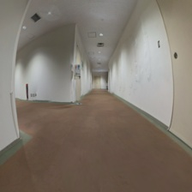
\includegraphics[width=15mm]{images/pf_obs3.png}};
\node[pic] (o2) at (-0.1,0.1) {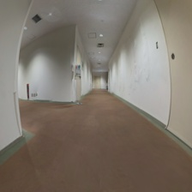
\includegraphics[width=15mm]{images/pf_obs2.png}};
\node[pic] (o1) at (-0.2,0.2) {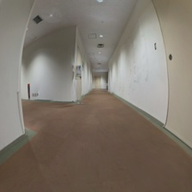
\includegraphics[width=15mm]{images/pf_obs1.png}};
\node[lbl, below=0.5mm of o3, align=center] {RGB images\\$4$ frames};

% ---- NoMaD 本体 ----------------------------------------------------------
\node[blk, frz] (enc) at (3.9,0) {Image encoder\\\small EfficientNet\text{-}B0, \frozen};
\node[blk, frz] (trn) at (7.8,0) {Transformer\\\small \frozen};
\node[circle, draw, inner sep=1.2pt] (sum) at (10.2,0) {$+$};
\node[blk, minimum width=21mm] (dif) at (13.5,0)
      {Diffusion policy\\\small $8$ waypoints};

% ---- 目標方向（本研究で追加）---------------------------------------------
% 直進・左折・右折のアイコン．この例では左折を与えているため，左折を強調する．
\def\diricon#1#2{\tikz[baseline=0, line width=1pt, rounded corners=1.1mm]
    \draw[-{Latex[length=1.8mm, width=2.1mm]}, #1] #2;}
\def\diricons{\diricon{}{(0,0) -- (0,4.2mm)}\quad
    \diricon{red, line width=1.8pt}{(0,0) |- (-2.9mm,3mm)}\quad
    \diricon{}{(0,0) |- (2.9mm,3mm)}}
\node[blk, fill=black!8, minimum width=21mm] (cmd) at (3.6,-1.7) {Target direction\\[0.5mm]\diricons};
\node[blk, fill=black!8] (den) at (7.8,-1.7) {Direction encoder\\\small 3\text{-}layer MLP};

% ---- 深度・障害物 --------------------------------------------------------
\node[blk, minimum width=18mm] (udp) at (3.6,-3.7) {\UniDepth};
\node[pic] (dep) at (6.6,-3.7) {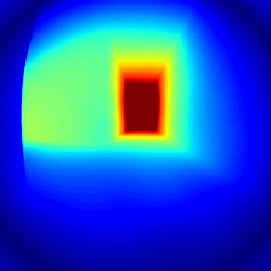
\includegraphics[width=13mm]{images/pf_depth_cmap.png}};
\node[pic] (bev) at (9.6,-3.7) {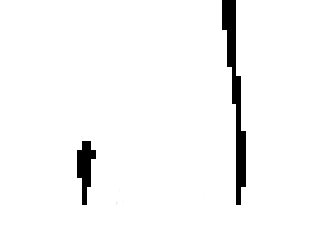
\includegraphics[height=13mm]{images/pf_bev_cc_noarrow.png}};
\draw (bev.south west) rectangle (bev.north east);
\node[lbl, below=0.5mm of bev] {BEV};

% ---- CARE ----------------------------------------------------------------
\node[blk] (care) at (13.5,-3.7) {\CARE};
\node[val] (vw)  at (17.95,-3.7) {$(v,\omega)$};

% ---- CARE による補正の模式図（例示）--------------------------------------
% 背景は BEV と同じ画像（幅 1.9 の座標系に合わせて軌道を重ねる）．
% scale で画像幅 2.4cm に合わせて座標系ごと拡大する．
\begin{scope}[shift={(16.75,-2.4)}, x=1cm, y=1cm, scale=2.4/1.9]
  \node[anchor=south west, inner sep=0pt] at (0,0)
        {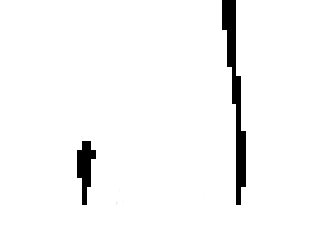
\includegraphics[width=2.4cm]{images/pf_bev_cc_noarrow.png}};
  \draw (0,0) rectangle (1.9,1.365);
  \draw[densely dashed, gray, thick] (0.96,0.17)
        .. controls (0.96,0.45) and (0.8,0.62) .. (0.3,0.68)
        node[lbl, below, inner sep=1.5pt] {$p_k$};
  \draw[thick] (0.96,0.17)
        .. controls (0.96,0.7) and (0.8,0.95) .. (0.2,1.0)
        node[lbl, pos=0.8, above, inner sep=1.5pt] {$p'_k$};
  \node[lbl, anchor=north] (toplab) at (0.95,0) {example};
\end{scope}
\coordinate (topsw) at (16.75,-2.4);

% ---- 結線 ----------------------------------------------------------------
\draw[ar] (o3) -- (enc);
\draw[ar] (enc) -- (trn);
\draw[ar] (trn) -- (sum);
\draw[ar] (sum) -- (dif);
\draw[ar] (cmd) -- (den);
\draw[ar] (den.east) -| (sum.south);
\draw[ar] (o1.west) -- ++(-0.35,0) |- (udp.west);
\draw[ar] (udp) -- (dep);
\draw[ar] (dep) -- (bev);
\draw[ar] (dif.south -| care.north) -- (care.north);
\draw[ar] (bev) -- (care);
\draw[ar] (care) -- (vw);
\draw[black!60, densely dashed, thick] (care.north east) -- (topsw);


% ---- 枠 ------------------------------------------------------------------
\begin{scope}[on background layer]
  \node[grp, fit=(enc)(dif)(cmd)(den), inner sep=3mm] (gn) {};
\end{scope}
\node[lbl, anchor=north west, fill=white, inner xsep=2pt]
      at ([xshift=2mm,yshift=0.2mm]gn.north west) {Direction\text{-}conditioned \NoMaD};
\end{tikzpicture}
}
  \caption{Path-following module}
  \label{fig:path_following}
\end{figure}

\subsection{学習}

学習は2段階で行い，視覚エンコーダは両段階を通じて凍結する．
目標方向の埋め込みは学習初期には十分に形成されていないため，第1段階では拡散モデルも凍結し，目標方向の埋め込みのみを学習する．
これにより，事前学習済みの拡散モデルを保持したまま，目標方向の埋め込みを学習する．
第2段階では拡散モデルの凍結を解き，小さい学習率で適合させる．

第1段階では，目標方向の埋め込みの学習率を$5\times10^{-4}$とし，20エポック学習する．
第2段階では，拡散モデルの学習率を$2\times10^{-6}$，目標方向の埋め込みの学習率を$5\times10^{-5}$とし，12エポック学習する．
いずれの段階も，バッチサイズを64とし，学習率はウォームアップの後にコサインスケジュールで減衰させる．
% TODO: 要確認．値は vnm_ros/config/experiments/nomad_yawfix_staged_stage1，stage2 の nomad.yaml から取った．
%       SI原稿の実験でこの設定の重みを用いたか確認する．

目標方向のラベルは直進に偏るため（\tabref{tab:dataset}），損失には各方向の出現頻度に応じた重みを与える．
目標方向$c$のサンプル数を$N_c$とすると，その重み$w_c$を
\begin{equation}
  w_c \propto N_c^{-1/2}
  \label{eq:loss_weight}
\end{equation}
とし，全サンプルにわたる重みの平均が1となるように正規化する．
出現頻度の逆数をそのまま用いると，サンプル数の少ない左折と右折の重みが大きくなりすぎるため，平方根をとって偏りを緩和する．

\subsection{推論と衝突回避}

推論時は，拡散モデルから複数のwaypoint列を生成してその平均を基準の軌道とし，障害物からの反発力に基づく衝突回避手法\CARE\cite{care}により補正する．
生成するwaypoint列は8本とし，拡散モデルの反復回数は10回とする．
\CARE には，\UniDepth が推定した深度から求めた前方近傍の点群を障害物として与える．
これにより，幾何情報に基づく安全性を付加することを狙う．
補正後の軌道上の1点を目標として選び，その方位から並進速度と角速度を算出する．

目標点のロボット座標系における位置を$(x, y)$，制御周期を$\Delta t$とすると，並進速度$v$と角速度$\omega$は次式で求める．
\begin{equation}
  v = \frac{x}{\Delta t}, \qquad
  \omega = \frac{1}{\Delta t}\arctan\frac{y}{x}
  \label{eq:control}
\end{equation}
これはViNTおよび\NoMaD の参照実装と同じ制御則である．
求めた速度は，並進速度$\SI{0.2}{m/s}$，角速度$\SI{0.3}{rad/s}$を上限として制限する．
% TODO: 要確認．制御周期（model_rate 3 Hz），速度の上限，目標点の番号は
%       vnm_ros/config/experiments/nomad_yawfix_staged_stage2/runtime.yaml，nomad.yaml，config/care.yaml から取った．
%       目標点の番号が nomad.yaml（waypoint_index: 2）と care.yaml（waypoint_index: 4）で異なるので，実験時の値を確認する．
